\section{Radionuclide Transport In Cyder}\label{sec:nuclide_models}


The results here provide an overview of the relative importance of thermal
parameters that affect the repository capacity of simplified generic
disposal concept in various geologic media where conduction is the dominant
heat transfer mode. The applicability of this sensitivity analysis is thus
restricted to enclosed, backfilled concepts.  

\subsection{Parametric Domain}

Sensitivity analyses were conducted which span the parametric range of values 
generated by the reference specific temperature change database and described 
in Table \ref{tab:thermal_cases}.  

\begin{table}[ht!]
\centering
\footnotesize{
\begin{tabular}{|l|l|l|r|}
\multicolumn{4}{c}{\textbf{Thermal Cases}}\\
\hline
\textbf{Parameter} & \textbf{Symbol} & \textbf{Units} & \textbf{Value Range} \\
\hline
Diffusivity & $\alpha_{th}$ & $[m^2\cdot s^{-1}]$ & $1.0\times10^{-7}-3.0\times10^{-6}$\\
\hline
Conductivity & $K_{th}$     & $[W\cdot m^{-1} \cdot K^{-1}]$ & $0.1 - 4.5$ \\
\hline
Spacing & $S$ & $[m]$ & 2, 5, 10, 15, 20, 25, 50 \\
\hline
Radius & $r_{lim}$ & $[m]$ & 0.1, 0.25, 0.5, 1, 2, 5 \\
\hline
Isotope & $i$ & $[-]$ & $^{241,243}Am,$  \\
        & & & $^{242,243,244,245,246}Cm,$  \\
        & & & $^{238,240,241,242}Pu$  \\
        & & & $^{134,135,137}Cs$  \\
        & & & $^{90}Sr$  \\
\hline
\end{tabular}
\caption{A thermal reference dataset of \gls{STC} values as a function of each of these parameters was generated by repeated parameterized runs of the LLNL 
MathCAD model\cite{greenberg_application_2012, greenberg_investigations_2012}.}
\label{tab:thermal_cases}
}
\end{table}



These values were selected to provide detail in the near field and at values of
$\alpha_{th}$ and $K_{th}$ in the three host media under consideration in this
work.

\subsection{Approach}

% used existing gdsms 
This analysis utilized the \gls{LLNL} semi-analytic MathCAD model
discussed in Section \ref{sec:llnl_background}.  It performs detailed
calculations of the conductive thermal transport in a generic repository
concept with a gridded layout.  

It relies on the thermal diffusivity, $\alpha_{th}$ and conductivity $K_{th}$ of 
the material as well as the waste package spacing, $S$, and thermally limiting 
radius, $r_{lim}$. Finally, it relies on the \gls{STC} data calculated with the 
semi-analytic model based on the decay heat profiles of the emplaced wastes, $Q$. 
The essential decay heat profiles, $Q$, were retrieved from a \gls{UFD} database 
provided by Carter et al. \cite{carter_fuel_2011}.



\subsection{Interfaces}
The interfaces between the models are essential to the understanding of the 
models themselves. The interfaces define boundary conditions in a number of 
forms based on information available internally to the component implementation. 

In a saturated, reducing environment, contaminants are transported by dispersion 
and advection. It is customary to define the combination of molecular diffusion 
and mechanical mixing as the dispersion tensor, $D$, such that, for a 
conservative solute, the mass conservation equation becomes 
\cite{schwartz_fundamentals_2004, wang_introduction_1982, 
van_genuchten_analytical_1982}:

    \begin{align}
      J &= J_{dis} + J_{adv}\nonumber\\
      &= -\theta(D_{mdis} + \tau D_m)\nabla C + \theta vC\nonumber\\ 
      &= -\theta D\nabla C + \theta vC \nonumber\\ 
      \intertext{which, for uniform flow in $\hat{k}$, is}
      &=\left(-\theta D_{xx} \frac{\partial C}{\partial x}
             \right)\hat{\imath}
             + \left( -\theta D_{yy} \frac{\partial C}{\partial y}
            \right)\hat{\jmath}
            + \left( -\theta D_{zz} \frac{\partial C}{\partial z}
             + \theta v_zC 
            \right)\hat{k},
      \label{unidirflow}
      \intertext{where}
      J_{dis} &= \mbox{ Total Dispersive Mass Flux }[kg/m^2/s]\nonumber\\
      J_{adv} &= \mbox{ Advective Mass Flux }[kg/m^2/s]\nonumber\\
      \tau &= \mbox{ Tortuosity }[-] \nonumber\\
      \theta &= \mbox{ Porosity }[\%] \nonumber\\
      D_m &= \mbox{ Molecular diffusion coefficient }[m^2/s]\nonumber\\
      D_{mdis} &= \mbox{ Coefficient of mechanical dispersivity}[m^2/s]\nonumber\\
      D &= \mbox{ Effective Dispersion Coefficient }[m^2/s]\nonumber\\
      C &= \mbox{ Concentration }[kg/m^3]\nonumber\\
      v &= \mbox{ Fluid Velocity in the medium }[m/s].\nonumber
    \end{align}

Solutions to this equation can be categorized by their boundary conditions and 
those boundary conditions serve as the interfaces between components in the 
\Cyder library of nuclide transport models.

  \begin{figure}[htp!]
    \begin{center}
      \def\svgwidth{\textwidth}
      \input{./chapters/methodology/nuclide_models/interfaces/flow.eps_tex}
    \end{center}
    \caption[\Cyder Component interfaces provide a source term  and three 
    boundary condition types.]{The boundaries between components (e.g., waste form and waste 
      package) are robust interfaces defined by boundary condition types.}
    \label{fig:flow}
  \end{figure}

In addition to a specified source term, the first, specified-head or Dirichlet type boundary conditions define a specified species 
concentration on some section of the boundary of the representative volume, 

    \begin{align}
      C(\vec{r},t)\Big|_{\vec{r} \in \Gamma} &= C_0(t)
      \intertext{where}
      \vec{r} &= \mbox{ position vector }\nonumber\\
      \Gamma &= \mbox{ domain boundary }.\nonumber
    \end{align}

The second type, specified-flow or Neumann type boundary conditions describe a full set of 
concentration gradients at the boundary of the domain,

    \begin{align}
      \frac{\partial C(\vec{r},t)}{\partial r}\Big|_{\vec{r}\in\Gamma} &= f(t)\\
      f(t) &= \mbox{ known function }.\nonumber
    \end{align}
    

The third, head-dependent mixed boundary condition or Cauchy type, defines a solute 
flux along a boundary. For a vertically oriented system with advective velocity 
in the $\hat{z}$ direction,

    \begin{align}
      -D\frac{\partial C(z, t)}{\partial z}\Big|_{z \in \Gamma} + v_zC(z, t) &= v_zC(t) 
      \intertext{where}
      C(t) &= \mbox{ a known concentration function }[kg/m^{3}].\nonumber
    \end{align}  

The spatial concentration throughout the volume is sufficient to fully describe 
implementation of the following nuclide transport models within \Cyder. This is 
supported by the implementation in which vertical advective velocity is uniform 
throughout the system and in which parameters such as the dispersion coefficient 
are known for each component. Since this is the case in \Cyder, description of 
the Dirichlet condition is sufficient to fully define calculation of the Neumann 
and Cauchy type conditions.



\subsection{Degradation Rate Radionuclide Transport Model}\label{sec:deg_rate}
The degradation rate model, simulating the fractional degradation of the 
material containment properties, is the simplest of implemented models and is most 
appropriate for simplistic waste package failure modeling. The fundamental 
concept is depicted in Figure \ref{fig:deg_volumes}.

\begin{figure}[h!]
  \begin{center}
    \def\svgwidth{.7\textwidth}
    \begin{figure}[h!]
  \begin{center}
    \def\svgwidth{.7\textwidth}
    \input{./chapters/methodology/nuclide_models/mass_balance/deg_rate/deg_volumes.eps_tex}
  \end{center}
  \caption[Constituents of a Degradation Rate Control Volume]{The control volume contains an 
  intact volume $V_i$ and a degraded volume, $V_d$. Contaminants in $V_d$ are 
  available for transport, while contaminants in $V_i$ are contained.}
  \label{fig:deg_volumes}
\end{figure}


  \end{center}
  \caption[Constituents of a Degradation Rate Control Volume]{The control volume contains an 
  intact volume $V_i$ and a degraded volume, $V_d$. Contaminants in $V_d$ are 
  available for transport, while contaminants in $V_i$ are contained.}
  \label{fig:deg_volumes}
\end{figure}



The materials that constitute the engineered barriers in a saturated 
repository environment degrade over time. The implemented model of this nuclide 
release behavior is based solely on a fractional degradation rate. 
The degraded volume is a simple fraction, $d$, of the total volume, $V_T$, such 
that 
\begin{align}
V_T &= V_i + V_d
\label{deg_volumes}
\intertext{where}
V_d(t) &= d(t)V_T\nonumber\\
V_i(t) &= (1-d(t))V_T\nonumber\\
V_T &= \mbox{ total volume }[m^3]\nonumber\\
V_i(t) &= \mbox{ intact volume at time t }[m^3]\nonumber\\
V_d(t) &= \mbox{ degraded volume at time t }[m^3]\nonumber
\intertext{and}
d(t) &= \mbox{ the fraction that has been degraded by time t }[-].\nonumber
\end{align}


\subsubsection{Calculation of Mass Transfer}
In this model, the contaminants in the degraded fraction of the control volume 
are available to adjacent components. The available contaminants
$m_{ij}(t)$, at the boundary between cell $i$ to cell $j$ at time $t$ are thus

\begin{align}
\dot{m}_{ij}(t) &= f_im_i(t)
\label{deg_rate_source_cont}
\intertext{where}
\dot{m}_{ij} &= \mbox{ the rate of mass transfer from i to j }[kg/s]\nonumber\\
f_i &= \mbox{ degradation rate function in cell i }[1/s] \nonumber\\
m_i &= \mbox{ mass in cell i }[kg] \nonumber\\
t &= \mbox{ time  }[s].\nonumber
\end{align}

For a situation as in \Cyder and \Cyclus, with discrete time steps, the time steps are 
assumed to be small enough to assume a constant rate $m_{ij}$ over the course 
of the time step. This model incorporates the source term made available on the 
inner boundary into its available mass and defines the resulting boundary 
conditions at the outer boundary as solely a function of the degradation rate 
of that component.  The mass transferred between discrete times $t_{n-1}$ and 
$t_n$ is thus a simple linear function of the transfer rate in 
\eqref{deg_rate_source_cont}, 

\begin{align}
m_{ij}(t_n) &= \int_{t_{n-1}}^{t_n}\dot{m}_{ij}(t')dt' \nonumber\\
         &= f_im_i(t_{n-1})\left[t_n - t_{n-1}\right].
\label{deg_rate_source_discrete}
\end{align}

\subsubsection{Boundary Interfaces}
\label{sec:dr_bc}
The mass $m_{df}(t_n)$ is the source term at the outer boundary, 
\begin{align}
  \mathcal{S}_j(t_n) &= \mbox{ fixed source term flux at }r_j [kg]\nonumber\\ 
                     &= m_{df}(t_n).
\end{align}
Thus, for the case in which all engineered barrier components are represented by 
degradation rate models, the source term at the outermost edge will be solely
a function of the original central source and the degradation rates of the 
components. 

The concentration boundary condition must also be defined at the outer boundary 
to support parent components that utilize the Dirichlet boundary condition. For 
the degradation rate model, which incorporates no diffusion or advection, the 
concentration, $C_j$ at $r_j$, the boundary between cells $j$ and $k$, is the average 
concentration in the saturated pore volume,

\begin{align}
\mathcal{D}_j(t_n) &= \mbox{ fixed concentration from component j at }t_n [kg/m^3].\nonumber\\ 
                   &= C_{j}(t_n)\nonumber\\ 
                   &= C_{df}\nonumber\\
                   &= \frac{m_{d}(t_n)}{V_{d}(t_n)}\\
\label{deg_rate_dirichlet}\\
&= \frac{\mbox{ solute mass in degraded fluid in cell j }}{\mbox{ degraded fluid volume in cell j}}.\nonumber 
\end{align}

To support parent components that utilize the Neumann boundary condition, the 
concentration gradient can be found if the concentration and the 
radial midpoint of the external component, $k$, are specified.

\begin{align}
\mathcal{N}_j(t_n) &= \mbox{ fixed concentration gradient from component j at }t_n [kg/m^3/s]\nonumber\\
                   &= \frac{dC(t_n)}{dr}\Bigg|_{r=r_j}\nonumber\\ 
                   &= \frac{C_k(r_{k-1/2},t_{n-1}) - C_j(r_{j-1/2}, t_n)}{r_{k-1/2} - r_{j-1/2}}
\label{neumann_dr}
\intertext{where}
r_{j-1/2} &= r_{j} - \frac{r_{j} - r_i}{2}\nonumber\\
r_{k-1/2} &= r_{k} - \frac{r_{k} - r_j}{2}.\nonumber
\end{align}


To support parent components that utilize the Cauchy boundary condition, the 
degradation rate model assumes that the fluid velocity is constant across the cell 
as is the concentration. Thus, 

\begin{align}
\mathcal{C}_j(t_n) &= \mbox{ fixed concentration flux from component j at }t_n [kg/m^2/s]\nonumber\\
                   &= -D\frac{\partial C(t_n)}{\partial r}\Bigg|_{r=r_j} + v_zC(t_n)\Bigg|_{r=r_j} \\
\label{deg_rate_cauchy}
            &= v_zC_0\nonumber
\intertext{where}
            C_0 &= \mbox{ a fixed concentration }[kg/m^3].\nonumber
\end{align}

%<++> &= \mbox{ <++> }[<++>] \nonumber\\


\section{Mixed Cell Volume Radionuclide Model}\label{sec:mixed_cell}

    % WF : glass 

      % alteration

      % temperature limit

    % WF : uox 

      % cladding limit

      % corrosion

A main nuclide transport component model used in this work is a mixed cell 
component module incorporating solubility and sorption effects as well as  
engineered material dissolution.

A graphical representation of the mixed cell model is given in Figures 
\ref{fig:intact} and \ref{fig:dissolved}.  

\begin{figure}[h!]
\begin{minipage}[b]{0.5\linewidth}
  \begin{center}
    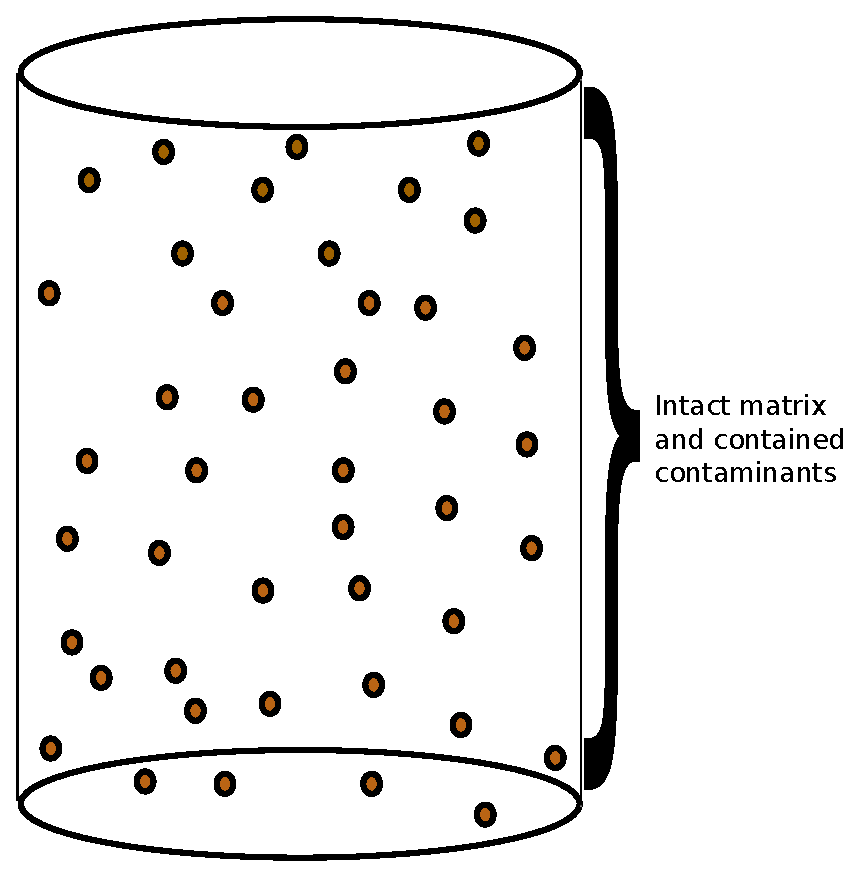
\includegraphics[height=7cm]{./chapters/nuclide_models/mixed_cell/mixed_cell_whole.eps}
  \end{center}
  \caption[Intact Mixed Cell Control Volume]{The control volume contains an 
  intact material matrix and contaminants that are unavailable to neighboring 
  subcomponents until dissolution has begun.}
  \label{fig:intact}
\end{minipage}
\hspace{0.5cm}
\begin{minipage}[b]{0.5\linewidth}
  \begin{center}
    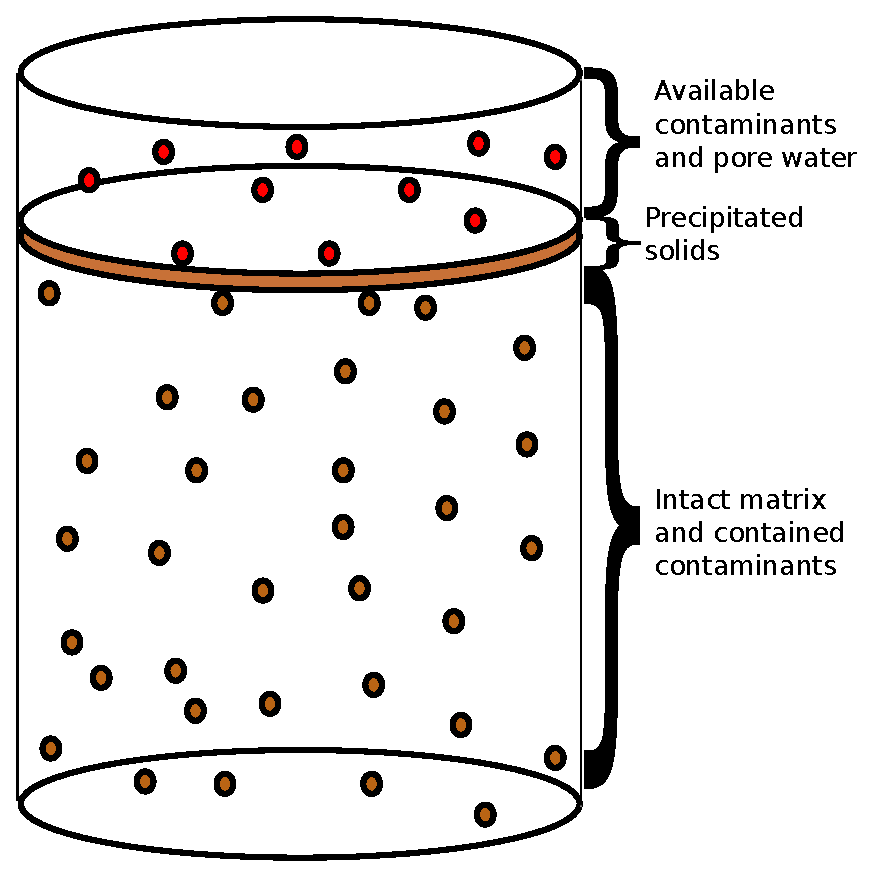
\includegraphics[height=7cm]{./chapters/nuclide_models/mixed_cell/mixed_cell_degraded.eps}
  \end{center}
  \caption[Degrading Mixed Cell Control Volume]{Once dissolution begins, the 
  :control volume contains a partially dissolved material matrix, contaminated 
  pore water, and precipitated solids.}
  \label{fig:dissolved}
\end{minipage}
\end{figure}


After some time degrading, the volume of free fluid can be expressed 
\begin{align}
V_{ff}(t_n) &= \theta V_T \int_{t_0}^{t_n} f(\cdots) dt.
\label{vff}
\end{align}

The volume of the intact matrix can be expressed
\begin{align}
V_{im}(t_n) &= V_T - V_T\int_{t_0}^{t_n} f(\cdots) dt.
\label{vim}
\end{align}

Finally, the volume of the precipitated solids can be expressed
\begin{align}
V_{ps}(t_n) &= (1 - \theta)V_T\int_{t_0}^{t_n} f(\cdots) dt.
\label{vps}
\end{align}

This model assumes that all net influx to the cell enters the free fluid rather 
than the intact matrix. The total volumetric contaminant concentration in the intact matrix, 
can be expressed

\begin{align}
C_{im}(t_n) &= C_0\\
            &= \frac{m_0}{V_{im}}
\intertext{where}
%here we assume nothing escapes an intact matrix
m_0 &= \mbox{ total initial mass } \nonumber
\end{align}

The resulting contaminant mass in the intact matrix is 

\begin{align}
m_{im}(t_n) &= C_0 V_{im}(t_n)\nonumber\\
            &= C_0(1-\theta) V_T\int_{t_0}^{t_n}f(\cdots)dt. 
\label{mim}
\end{align}

The contaminant mass in the free fluid is just the pore water concentration 
times the free fluid volume plus the time integral of net influx to the cell. 

\begin{align}
C_{ffT}(t_n) &= \left[C_0 + \frac{\int_{t_0}^{t_n} \dot{m}_{i}(t') dt'}{V_{ff}(t_n)}\right] 
\intertext{and}
m_{ffT}(t_n) &= C_{ff}(t_n)\theta V_{ff}(t_n)\nonumber\\
       &= \left[C_0 + \frac{\int_{t_0}^{t_n} \dot{m}_{i}(t') dt'}{V_{ff}(t_n)}\right] V_{ff}(t_n) \nonumber\\
       &= C_0V_{ff}(t_n) + \int_{t_0}^{t_n} \dot{m}_{i} dt'
\end{align}

It is limited, however, by both solubility limitation and sorption. 

\subsection{Sorption}

The mass in both the free fluid and in the intact matrix exists in both 
sorbed and nonsorbed phases. The relationship between the sorbed mass 
concentration in the solid phase (e.g. the pore walls),

\begin{align}
s &=\frac{\mbox{ mass of sorbed contaminant} }{ \mbox{mass of total solid phase }}
\label{solid_conc}
\end{align}
and the dissolved liquid concentration, 
\begin{align}
c &=\frac{\mbox{ mass of dissolved contaminant} }{ \mbox{volume of total liquid phase }}
\label{liquid_conc}
\end{align}
can be expressed by a number of isotherm models.

In this model, sorption is taken into account throughout the volume. In the 
intact matrix, the contaminant mass is distributed between the pore walls and 
the pore fluid by sorption.  So too, contaminant mass released from the intact 
matrix by degradation is distributed between dissolved mass in the free fluid 
and sorbed mass in the precipitated solids.


\subsection{Boundary Conditions}

To solve for the boundary condiitons in this model, the amount of dissolved mass 
in the free fluid must be found. This value, $m_{ffl}$, can be expressed in terms of the 
total degraded contaminant mass and the contaminant mass in the precipitated 
solid,

\begin{align}
m_{ffl} &= m_{ffT} - m_{psc}
\label{m_ffl}
\end{align}

The mass of contaminant sorbed into the precipitated solids can be found using a 
linear isotherm model, characterized by the relationship 
\begin{align}
s_{i} &= K_{di} c_{i}
\label{linear_iso}
\intertext{where}
s_i &= \mbox{ the solid concentration of isotope i }[kg/kg]\nonumber\\
K_{di} &= \mbox{ the distribution coefficient of isotope i}[]\nonumber\\
c_i &= \mbox{ the liquid concentration of isotope i }[kg/m^3].\nonumber
\end{align}

Thus, 

\begin{align}
s_{i,ps} &= \frac{\mbox{contaminant mass in precipitated solids} }{ \mbox{total mass of precipitated solids}}\nonumber\\
         &= \frac{m_{psc}}{m_{pst}}\nonumber\\
         &= \frac{m_{psc}}{m_{psm} + m_{psc}}\nonumber\\
\intertext{where}
m_{psm}  &= \mbox{ noncontaminant mass in precipitated solids }[kg]\nonumber\\
         &= \rho_bV_{ps}\nonumber\\
m_{psc}  &= \mbox{ contaminant mass in precipitated solids }[kg]\nonumber\\
m_{psm}  &= \rho_bV_{ps}.
\label{s_ps}
\end{align}

The following expression results, giving contaminant mass in the precipitated 
solids in terms of the sorption coefficient,
\begin{align}
m_{psc} &= s_{ps}m_{psT}\nonumber\\
          &= K_dC_{ffl}m_{psT}\nonumber\\
          &= \frac{K_dm_{ffl}m_{psT}}{V_{ff}}\nonumber\\
          &= \frac{K_d}{V_{ff}}(m_{ffT}-m_{psc})m_{psT}\nonumber\\
          &= \frac{K_d}{V_{ff}}(m_{ffT}-m_{psc})(m_{psm}+m_{psc})\nonumber\\
          &= \frac{K_d}{V_{ff}}(m_{ffT}m_{psm}-m_{psc}m_{psm} + m_{ff}m_{psc} -m_{psc}^2)\nonumber\\
          &= \frac{K_d}{V_{ff}} (m_{ffT}m_{psm} + (m_{ffT} - m_{psm})m_{psc} - m_{psc}^2)\nonumber
\intertext{which, rearranged, becomes }
0         &= m_{psc}^2 + \left( -m_{ffT} + m_{psm} + \frac{V_{ff}}{K_d} \right)m_{psc} - m_{ffT}m_{psm}\nonumber
\intertext{and is solved using the quadratic formula, such that}
m_{psc}   &= \frac{m_{ffT} - m_{psm} - \frac{V_{ff}}{K_d}}{2} \nonumber\\
          & \pm\frac{\sqrt{m_{ffT}^2 + m_{psm}^2 + \frac{V_{ff}^2}{K_d^2} + 2m_{ffT}m_{psm} - 
             \frac{2V_{ff}m_{ffT}}{K_d} + \frac{2V_{ff}m_{psm}}{K_d} } }{2} \nonumber
\intertext{which, again rearranged, becomes}
          &= \frac{1}{2} \left(m_{ffT} - m_{psm} - \frac{V_{ff}}{K_d}\right) \nonumber\\
          & \pm \frac{1}{2} \sqrt{m_{ffT}^2 + 2m_{ffT}\left(m_{psm} - 
          \frac{V_{ff}}{K_d}\right) + \left(m_{psm} + 
          \frac{V_{ff}}{K_d}\right)^2}.
\label{m_psc}
\end{align}

If we plug Equation \eqref{m_psc} into Equation \eqref{m_ffl}, we arrive at the 
following expression for $m_{ffl}$ in terms of known quantities

\begin{align}
m_{ffl}   &= m_{ffT} - \frac{1}{2} \left(m_{ffT} - m_{psm} - \frac{V_{ff}}{K_d}\right) \nonumber\\
          & \mp \frac{1}{2} \sqrt{m_{ffT}^2 + 2m_{ffT}\left(m_{psm} - 
          \frac{V_{ff}}{K_d}\right) + \left(m_{psm} + 
          \frac{V_{ff}}{K_d}\right)^2}.
\label{m_ffl_full}
\end{align}

We can express the desired boundary conditions in terms of $m_{ffl}$. First, the 
Dirichlet boundary condition is 
\begin{align}
C(x,y,z,t) = \frac{m_{ffl}(t)}{V_{ff}(t)}\forall (x,y,x) \in \Gamma.
\label{dirichlet_mixed}
\end{align}

Again, the concentration gradient can be specified across the boundary only with 
reference to the concentration at a point external to the component. 
If the concentration $C_{ext}$ is specified at a location $r_{ext}$, the Neumann 
condition is a function of those concentrations, $C(x,y,z,t)$, and a 
corresponding location inside the component. If we choose radius furthest from 
either wall of the inner component, $r_c$, 

\begin{align}
\frac{\partial C}{\partial r} = \frac{C_{ext} - C(x,y,z,t)}{r_{ext} - r_{c}}&
\label{neumann_mixed}
\intertext{such that}
\theta_i\vec{v_i}(t) C(x,y,z,t) \frac{C_{ext} - C(x,y,z,t)}{r_{ext} - r_{c}} &= \theta_i\vec{v_i}(t) C(x,y,z,t).
\end{align}





\subsubsection{Lumped Parameter Radionuclide Mass Balance Model}\label{sec:lumped}

For systems in which the flow is sufficiently slow to be assumed constant over 
a time step, it is possible to model a system of volumes as a connected lumped 
parameter models (Figure \ref{fig:lumpedseries}). 
The Lumped Parameter mass balance model implements a response function model 
based on this lumped parameter interpretation and capable of Piston Flow, 
Exponential, and Dispersion response functions from Maloszewski and Zuber 
\cite{maloszewski_lumped_1996}.

\begin{figure}[htbp!]
  \begin{center}
    \def\svgwidth{.8\textwidth}
    \input{./chapters/methodology/nuclide_models/mass_balance/lumped/lumpedseries.eps_tex}
  \end{center}
  \caption{A system of volumes can be modeled as lumped parameter models in 
  series.}
  \label{fig:lumpedseries}
\end{figure}

Each lumped parameter component is modeled according to a 
relationship between the incoming concentration, $C_{in}(t)$, and the outgoing 
concentration, $C_{out}(t)$, 

\begin{align}
  C_{out}(t) &= \int_0^\infty C_{in}(t-t')g(t')e^{-\lambda t'}dt'
  \label{lumped2}
  \intertext{where}
  t'  &= \mbox{ transit time }[s]\nonumber\\
  g(t')  &= \mbox{ response function, a.k.a. transit time distribution}[-]\nonumber]\\
  \lambda &= \mbox{ radioactive decay constant }[s^{-1}].\nonumber
\end{align}

Selection of the response function is usually based on experimental tracer 
results in the medium at hand. If such data is available, functions used 
commonly in chemical engineering applications \cite{maloszewski_lumped_1996} 
include the Piston Flow Model (PFM), 

\begin{align}
  g(t') &= \delta{(t'-t_t))}
  \intertext{ the Exponential Model (EM) }
  g(t') &= \frac{1}{t_t}e^{-\frac{t'}{t_t}}
  \intertext{ and the Dispersion Model (DM), }
  g(t') &= \left( \frac{\emph{Pe }t_t}{4\pi t'} \right)^{\frac{1}{2}}
  \frac{1}{t'}e^{- \frac{\emph{Pe }t_t\left( 1- \frac{t'}{t_t}  \right)^2} 
  {4t'}}, \intertext{where}
  \emph{Pe}  &= \mbox{ Peclet number for mass diffusion }[-]\nonumber\\
  t_t  &= \mbox{ mean tracer age }[s]\nonumber\\
    &= t_w \mbox{ if there are no stagnant areas }\nonumber\\
  t_w  &= \mbox{ mean residence time of water }[s]\nonumber\\
       &= \frac{V_m}{Q}\nonumber\\
       &= \frac{z}{v_z}\nonumber\\
       &= \frac{z\theta_e}{q}\nonumber
  \intertext{in which}
  V_m  &= \mbox{ mobile water volume }[m^3]\nonumber\\
  Q    &= \mbox{ volumetric flow rate }[m^3/s]\nonumber\\
  z    &= \mbox{ average travel distance in flow direction }[m]\nonumber\\
  v_z  &= \mbox{ mean water velocity}[m/s]\nonumber\\
  q    &= \mbox{ Darcy Flux }[m/s]\nonumber\\
  \theta_e &= \mbox{ effective (connected) porosity }[\%].\nonumber
\end{align}

The latter of these, the Dispersion Model satisfies the one dimensional 
advection-dispersion equation, and is therefore the most physically relevant for 
this application. The solutions to these for constant concentration at the 
source boundary are given in Maloszewski and Zuber \cite{maloszewski_lumped_1996}, 

\begin{align}
  C_{out}(t) &=\begin{cases}
    PFM & C_0e^{-\lambda t_t}\\
    EM  & \frac{C_0}{1+\lambda t_t}\\
    DM & C_0e^{\frac{\emph{Pe}}{2}\left(1-\sqrt{1+\frac{4\lambda 
    t_t}{\emph{Pe}}}\right)}.
  \end{cases}
  \label{lumpedsolns}
\end{align}

Since \Cyclus handles decay outside of \Cyder, the use of these models relies on a 
reference transit time and decay constant supplied by the user. The behavior of 
the reference isotope, in this way, fully defines the behavior of all isotopes.

It is important to note that a linear concentration profile is assumed between 
the inlet and the outlet,

\begin{align}
  C(z,t) = C_{in}(t)  + \frac{C_{out}(t) - C_{in}(t)}{z_{out} - z_{in}}z.
\end{align}


\subsection{One Dimensional Permeable Porous Medium Radionuclide Transport 
Model}\label{sec:one_dim_ppm}
Finally, abstraction results informed modifications to the implementation of an 
analytic solution to the one dimensional advection-dispersion equation with 
finite domain and Cauchy and Neumann boundary conditions at the inner and outer 
boundaries, respectively. 

Various solutions to the advection dispersion equation  
\eqref{unidirflow} have been published for both the first and third types of 
boundary conditions. The third, Cauchy type, is mass conservative, and will be 
the primary kind of boundary condition used at the source for this model.

The conceptual model in Figure \ref{fig:1dinf} represents solute transport in 
one dimension with unidirectional flow upward (a conservative assumption) and a 
semi-infinite boundary condition in the positive flow direction. The solution is 
given (Leij et. al, \cite{leij_analytical_1991}) and described below.  

\begin{figure}[h!]
  \begin{center}
    \def\svgwidth{.5\textwidth}
    \input{./chapters/methodology/nuclide_models/one_dim_ppm/1dinf.eps_tex}
  \end{center}
  \caption{A one dimensional, semi-infinite model, unidirectional flow,
  solution with Cauchy and Neumann boundary conditions}
  \label{fig:1dinf}
\end{figure}

For the boundary conditions, 
\begin{align}
  -D \frac{\partial C}{\partial z}\big|_{z=0} + v_zc &= \begin{cases}
    v_zC_0  &  \left( 0<t<t_0 \right)\\
    0  &  \left( t>t_0 \right)\\
  \end{cases},\\
  \frac{\partial C}{\partial z}\big|_{z=\infty} &= 0
  \intertext{and the initial condition,}
  C(z,0) &= C_i,
  \label{1dinfBC}
  \intertext{the solution is given as }
  C(z,t) = \frac{C_0}{2}\Bigg[&\mbox{erfc}\left[{\frac{L-v_zt}{2\sqrt{D_Lt}}}\right] 
  + \frac{1}{2} \left(\frac{v_z^2t}{\pi D_L}\right)^{1/2}e^{\frac{-( L - 
  v_zt)^2}{4D_Lt}}\nonumber\\
  &- \frac{1}{2}\left( 
  1+\frac{v_zL}{D_L}+\frac{v_z^2t}{D_L}\right)e^\frac{v_zL}{D_L}\mbox{erfc}\left[\frac{L-V_zt}{2\sqrt{D_Lt}}\right]
  \Bigg].
\end{align}




\subsection{Implications For Waste Form Modeling}

Though the Waste Form Component can be modeled by any of the available 
NuclideModels, the Degradation Rate based or Mixed Cell radionuclide transport 
models are preferred for modeling of the Waste Form Component.  This is 
because, in repository performance asessments, waste form dissolution is 
typically modeled as instantaneous or rate based. Dissolution related release 
is historically modeled as congruent, solubility limited, or both, with some 
radionuclides becoming immediately accessible, and some tending to remain in 
the fuel matrix. 

\subsection{Implications For Waste Package Modeling}

Though the Waste Package Component can be modeled by any of the available 
NuclideModels, the simple Degradation Rate based model is strongly preferred.
Waste package time to failure is dependent on water contact and heat, 
but is historically modeled probabilistically, or at a constant rate.
Accordingly, waste package degradation in repository performance is either 
neglected entirely, instantaneous and complete (a delay before full release), 
or partial and constant (a constantly present hole in the package). 


\subsection{Implications For Buffer Modeling}

Diffusion is the primary mechanism for nuclide transport through the 
buffer Component of the repository system. While the buffer may degrade, the 
near field has historically been modeled in as much hydrologic detail as 
possible. For this reason, the Lumped Parameter or One Dimensional Permeable 
Porous Medium nuclide transport models are preferred.

\subsection{Implications for Geologic Environment Modeling}

In most of the saturated, low permeability environments being considered, 
diffusion is the primary mechanism for nuclide transport through the geologic 
medium Component of the repository system. While the near field may degrade, 
the far field should be modeled in detail if possible. For this reason, the 
One Dimensional Permeable Porous Medium nuclide transport 
model is preferred.
